\begin{figure}[htbp]
\centering
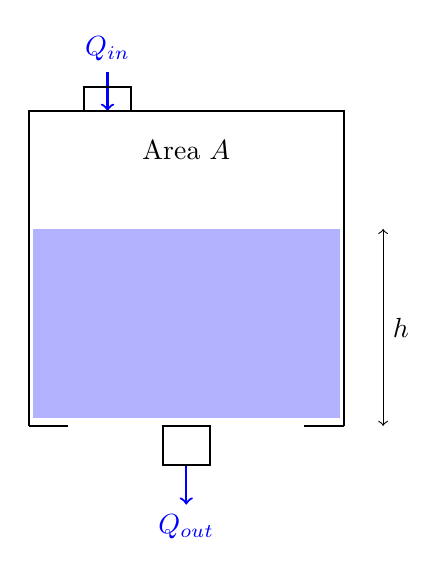
\begin{tikzpicture}
    % Tank
    \draw[thick] (0,0) -- (0,4) -- (4,4) -- (4,0);
    \draw[thick] (0,0) -- (0.5,0) (3.5,0) -- (4,0);

    % Liquid
    \fill[blue!30] (0.05,0.1) rectangle (3.95,2.5);

    % Level
    \draw[<->] (4.5,0) -- (4.5,2.5) node[midway, right] {$h$};

    % Inflow
    \draw[->, thick, blue] (1,4.5) -- (1,4) node[above, pos=0] {$Q_{\text{in}}$};
    \draw[thick] (0.7,4) rectangle (1.3,4.3);

    % Outflow
    \draw[->, thick, blue] (2,-0.5) -- (2,-1) node[below] {$Q_{\text{out}}$};
    \draw[thick] (1.7,-0.5) rectangle (2.3,0);

    % Area
    \node at (2,3.5) {Area $A$};
\end{tikzpicture}
\caption{Single tank level system.}
\label{fig:tank_level}
\end{figure}
